\documentclass{standalone}

\usepackage{tikz}
\usetikzlibrary{calc}
\usetikzlibrary{shapes}

\begin{document}
	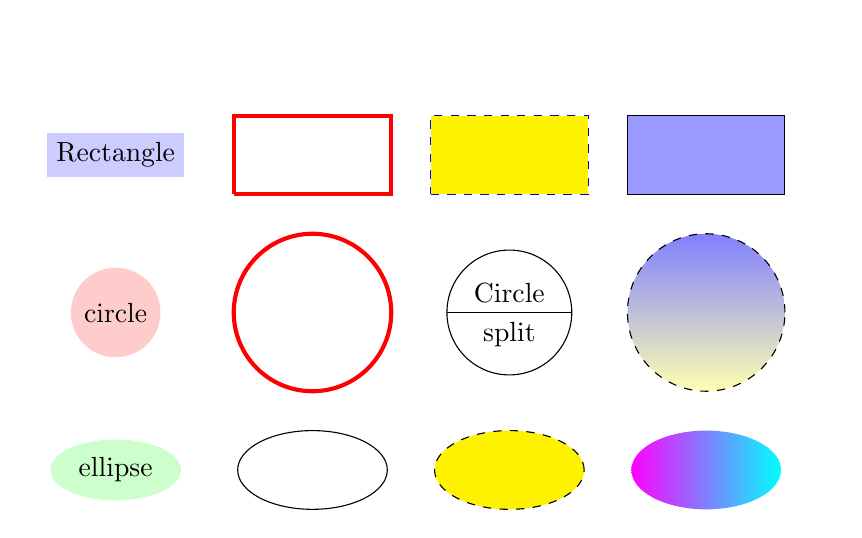
\begin{tikzpicture}

		\def \xmax{10};
		\def \ymax{3};

		\node[anchor=center, fill=none] (origemXY) at (0,0) {};
		\node[anchor=center] (fimXY) at (\xmax, \ymax) {};

		\coordinate (myrect) at (0.1*\xmax, 0.5*\ymax);
		\node[rectangle, fill=blue!20] (rect) at (myrect) {Rectangle};
		
		\coordinate (myrect2) at ($(myrect.west)+(2.5,0)$);
		\coordinate (myrect3) at ($(myrect2.west)+(2.5,0)$);
		\coordinate (myrect4) at ($(myrect3.west)+(2.5,0)$);
		
		\def \ladox{2};
		\def \ladoy{1};
		
		\draw[draw=red, line width=1.5pt] ($(myrect2)+(-0.5*\ladox,-0.5*\ladoy)$) -- ($(myrect2)+(0.5*\ladox,-0.5*\ladoy)$) -- ($(myrect2)+(0.5*\ladox,0.5*\ladoy)$) -- ($(myrect2)+(-0.5*\ladox,0.5*\ladoy)$) -- ($(myrect2)+(-0.5*\ladox,-0.5*\ladoy)$);
		
		\draw[dashed, draw=blue, fill=yellow] ($(myrect3)+(-0.5*\ladox,-0.5*\ladoy)$) -- ($(myrect3)+(0.5*\ladox,-0.5*\ladoy)$) -- ($(myrect3)+(0.5*\ladox,0.5*\ladoy)$) -- ($(myrect3)+(-0.5*\ladox,0.5*\ladoy)$) -- cycle;
		
		\filldraw[fill=blue!40!white, draw=black, anchor=west] ($(myrect4)+(-0.5*\ladox,-0.5*\ladoy)$) rectangle ($(myrect4)+(0.5*\ladox,0.5*\ladoy)$);
		
		
		\coordinate (mycircle) at ($(myrect.south)+(0, -2)$);
		\node[circle, fill=red!20] at (mycircle) {circle};
		
		\coordinate (mycircle2) at ($(mycircle.west)+(2.5,0)$);
		\coordinate (mycircle3) at ($(mycircle2.west)+(2.5,0)$);
		\coordinate (mycircle4) at ($(mycircle3.west)+(2.5,0)$);
		
		\def \raio{1};
		\draw[draw=red, line width=1.5pt] (mycircle2) circle (\raio);
		
		\node[circle split, draw=black ] (myci2) at(mycircle3) {Circle \nodepart{lower} split};
		\node[circle, draw=black, dashed, top color=blue!50, bottom color=yellow!30, minimum size=2*\raio cm, inner sep=0cm] (myci3) at(mycircle4) {};
		
		
		\coordinate (myellipse) at ($(mycircle.south)+(0, -2)$);
		\node[ellipse, fill=green!20] at (myellipse) {ellipse};
		
		\coordinate (myellipse2) at ($(myellipse.west)+(2.5,0)$);
		\coordinate (myellipse3) at ($(myellipse2.west)+(2.5,0)$);
		\coordinate (myellipse4) at ($(myellipse3.west)+(2.5,0)$);

		\def \ladoEx{0.95};
		\def \ladoEy{0.5};	
		
		\draw (myellipse2) ellipse (\ladoEx cm and \ladoEy cm);
		\node[circle, draw=black, xscale=2*\ladoEx cm, yscale=2*\ladoEy cm, inner sep=0cm, fill=yellow, dashed] (myel3) at(myellipse3) {};
		
		\draw (myellipse4) node[ellipse, minimum height=2*\ladoEy cm,minimum width=2*\ladoEx cm,draw=none, left color=magenta, right color=cyan] {};

	
	\end{tikzpicture}

\end{document}
